\documentclass[12pt,reqno]{amsart}
\usepackage{amsthm,amsmath,amssymb}
\usepackage{mathtools}
\usepackage{proof}
\usepackage{centernot}
\usepackage{xcolor}
\usepackage{graphicx}
\usepackage[T1]{fontenc}
\usepackage{courier}
\usepackage{enumitem}
\usepackage{array}
\usepackage{multirow}
\usepackage{listings}
\lstset{basicstyle=\ttfamily\small, columns=fullflexible, language=sql}
\definecolor{mySucces}{RGB}{40, 167, 69}
\definecolor{myFail}{RGB}{220, 53, 69}

\newcommand{\code}[1]{\texttt{#1}}
\newcommand{\st}[0]{\text{ s.t. }}
\newcommand{\where}[0]{\text{ where }}
\newcommand{\mand}[0]{\text{ and }}
\newcommand{\msgspc}[0]{\mathcal{M}}
\newcommand{\cphspc}[0]{\mathcal{C}}
\newcommand{\keyspc}[0]{\mathcal{K}}
\newcommand{\advrs}[0]{\mathcal{A}}
\newcommand{\oracle}[0]{\mathcal{O}}
\newcommand{\correctans}[0]{\colorbox{mySucces}{CORRECT}}
\newcommand{\falseans}[0]{\colorbox{myFail}{FALSE}}
\newcommand\MyBox[2]{
  \fbox{\lower0.75cm
    \vbox to 1.7cm{\vfil
      \hbox to 1.7cm{\hfil\parbox{1.4cm}{#1\\#2}\hfil}
      \vfil}%
  }%
}
\graphicspath{ {./} }
\newtheorem{theorem}{Theorem}[section]
\newtheorem{axiom}[theorem]{Axiom}
\newtheorem{case}[theorem]{Case}
\newtheorem{claim}[theorem]{Claim}
\newtheorem{conclusion}[theorem]{Conclusion}
\newtheorem{condition}[theorem]{Condition}
\newtheorem{conjecture}[theorem]{Conjecture}
\newtheorem{corollary}[theorem]{Corollary}
\newtheorem{criterion}[theorem]{Criterion}
\newtheorem{definition}[theorem]{Definition}
\newtheorem{example}[theorem]{Example}
\newtheorem{exercise}[theorem]{Exercise}
\newtheorem{lemma}[theorem]{Lemma}
\newtheorem{notation}[theorem]{Notation}
\newtheorem{problem}[theorem]{Problem}
\newtheorem{proposition}[theorem]{Proposition}
\newtheorem{remark}[theorem]{Remark}
\newtheorem{solution}[theorem]{Solution}
\newtheorem{summary}[theorem]{Summary}    
\begin{document}

\begin{center}
\large\textbf{Homework 2 \\ COMP530 Fall 2020 - Data Privacy and Security \\}
\normalsize\textbf{ Erhan Tezcan 0070881 \\ 05.12.2020} \\
\end{center}

\begin{center}
\line(1,0){250}
\end{center}

%
%\begin{enumerate}[label=\alph.]
% \item Explain input, output, and the purpose of each algorithm (Key Generation, Encryption, Decryption). 
% \item What are the key space, the message space, and the ciphertext space?
% \item Formally define the   correctness   requirement of an encryption scheme.
% \end{enumerate}
%

%	\begin{lstlisting}[language=sql]
%REVOKE ALL
%ON *
%FROM Frank
%	\end{lstlisting}

\section*{Answers}
\textbf{Answer 1:} There are 4 equivalence classes (EC). The questions $1.b$ to $1.h$ will be answered in the following list for each EC, and the remaining answers will follow. All of the values here are obtained by running \code{q1.py}, which also outputs these answers prettily to the console.
\begin{enumerate}
 \item $EC_1 = \{r_1, r_4, r_5, r_9, r_{13}, r_{16}\}$. It is an EC of QIs Teacher, Male, $[50, 60)$. It has SIs Flu (x2), HIV (x1), Diabetes (x3).
 \begin{itemize}
 	\item This EC is at most $6$-anonymous.
 	\item This EC is at most distinct $3$-diverse.
 	\item This EC is at most entropy $1.6688$-diverse.
 	\item This EC is at most recursive $(1,2)$-diverse.
 	\item This EC is at most recursive $(1.0,2)$-diverse.
 	\item This EC is at least $0.1470$-close with variational distance.
 	\item This EC is at least $0.0279$-close with Kullback-Leibler divergence.
 \end{itemize}
 \item $EC_2 = \{r_2, r_{11}, r_{14}\}$. It is an EC of QIs Teacher, Female, $[50, 60)$. It has SIs Flu (x1), HIV (x1), Diabetes (x1).
  \begin{itemize}
 	\item This EC is at most $3$-anonymous.
 	\item This EC is at most distinct $3$-diverse.
 	\item This EC is at most entropy $1.4999$-diverse.
 	\item This EC is at most recursive $(1,2)$-diverse.
 	\item This EC is at most recursive $(0.5,2)$-diverse.
 	\item This EC is at least $0.0392$-close with variational distance.
 	\item This EC is at least $0.0015$-close with Kullback-Leibler divergence.
 \end{itemize}
 \item $EC_3 = \{r_3, r_6, r_8, r_{17}\}$. It is an EC of QIs Carpenter, Male, $[40, 50)$. It has SIs Flu (x1), HIV (x2), Diabetes (x1).
  \begin{itemize}
 	\item This EC is at most $4$-anonymous.
 	\item This EC is at most distinct $3$-diverse.
 	\item This EC is at most entropy $1.6329$-diverse.
 	\item This EC is at most recursive $(1,2)$-diverse.
 	\item This EC is at most recursive $(1.0,2)$-diverse.
 	\item This EC is at least $0.2058$-close with variational distance.
 	\item This EC is at least $0.0379$-close with Kullback-Leibler divergence.
 \end{itemize}
 \item $EC_4 = \{r_7, r_{10}, r_{12}, r_{15}\}$. It is an EC of QIs Painter, Female, $[30, 40)$.  It has SIs Flu (x2), HIV (x1), Diabetes (x1).
  \begin{itemize}
 	\item This EC is at most $4$-anonymous.
 	\item This EC is at most distinct $3$-diverse.
 	\item This EC is at most entropy $1.6329$-diverse.
 	\item This EC is at most recursive $(1,2)$-diverse.
 	\item This EC is at most recursive $(1.0,2)$-diverse.
 	\item This EC is at least $0.1470$-close with variational distance.
 	\item This EC is at least $0.0202$-close with Kullback-Leibler divergence.
 \end{itemize}
\end{enumerate}
The questions $1.i$ to $1.k$ are answered in the following list:
 \begin{itemize}
 	\item The table is $k$-anonymous for $k \leq 3$.
 	\item The table is entropy $l$-diverse for $l \leq 1.4999$.
 	\item The table is $t$-close for $t \geq 0.2058$ with variational distance.
 \end{itemize}

\newpage
\textbf{Answer 2:} We know that for an EC $q^*$, $p(q^*, s)$ is the fraction of records in $q^*$ with $SA=s$. In probabilistic $l$-diversity, $\forall s \in SA$ we have:
$$
p(q^*, s) \leq \frac{1}{l}
$$ 
Let us denote $|q^*|$ as the number of records in EC $q^*$, and $|q_s^*|$ as the number of records in EC $q^*$ for some sensitive attribute $s$.
$$
\frac{|q_s^*|}{|q^*|}\leq \frac{1}{l}
$$ 
Equivalently, $ l\times|q_s^*|\leq |q^*|$.
\begin{itemize}[label=]
	\item \textbf{(a)} This is \textbf{true}.
	\begin{proof} Let EC $q^*$ be a probabilistic $l$-diverse dataset for some set of sensitive attributes $SA$. Then, $\forall s \in SA$ we have
	$$
	l\times|q_s^*|\leq |q^*|
	$$
	If we sum these inequalities for all possible values of $s$ we have:
	$$
	\sum_{s \in SA}l\times|q_s^*| \leq \sum_{s \in SA}|q^*|
	$$
	Dividing both sides by $l$ yields:
	$$
	\sum_{s \in SA}|q_s^*| \leq \frac{|SA|\times|q^*|}{l}
	$$
	Notice that $\sum_{s \in SA}|q_s^*| = |q^*|$ because that is basically the number of records for all SA values in this EC. So we have:
$$
	|q^*| \leq \frac{|SA|\times|q^*|}{l}
	$$
	The $|q^*|$ cancels out,
	$$
	1\leq \frac{|SA| }{l}
	$$
	Finally:
	$$
	l \leq |SA|
	$$
	This means that you have at least $l$ members in $SA$, which also means that you have at least $l$ distinct significant attributes, which implies that this EC is $l$-diverse.
	\end{proof}
 	\item \textbf{(b)} This is \textbf{false}.
 	\begin{proof} We can show this by giving a counter example. Imagine a 3-diverse EC $q^*$  where the set of sensitive attributes $SA = \{s_1, s_2, s_3\}$ and $|q_{s_1}^*|=8$, $|q_{s_2}^*|=1$, $|q_{s_3}^*|=1$, and $|q^*|=10$. For $s_1$ we have:
 $$
\frac{|q_{s_1}^*|}{|q^*|} = \frac{8}{10}\leq \frac{1}{3}
$$
We see that $24/30 \leq 10/30$ is false, so this is wrong. Even though the table is distinct 3-diverse it is not probabilistic 3-diverse.
\end{proof}
\item \textbf{(c)} This is \textbf{true}. 
\begin{proof}
In a single generalization step $D \rightarrow D'$, new ECs are created by merging existing ECs. Let us look at such case, where two ECs, namely $q^L$ and $q^R$, are merged into $q^N$. Suppose that the table is probabilistic $l$-diverse with set of sensitive attributes $SA$. This implies both $q^L$ and $q^R$ are probabilistic $l$-diverse. We will see what the diversity might be for $q^N$. 

Similar to what we have shown in the proof of first part of this question, realize that
\begin{equation}
|q^L| \leq \frac{|SA|\times|q^L|}{l}
\end{equation}
and
\begin{equation}
|q^R| \leq \frac{|SA|\times|q^R|}{l}
\end{equation}
When these two are merged into $q^N$, for probabilistic $l$-diversity we require:
$$
|q^N| \leq \frac{|SA|\times|q^N|}{l}
$$
Notice that $|q^N| = |q^L| + |q^R|$. Thus,
$$
|q^L| + |q^R| \leq \frac{|SA|\times|q^L|}{l} + \frac{|SA|\times|q^R|}{l}
$$
We can see that this is infact a true inequality, because it is actually sum of inequalities in equations (1) and (2). This shows that generalization can not result in a dataset that has less probabilistic $l$-diversity, so we can say that generalization is monotonic with respect to probabilistic $l$-diversity.
\end{proof}
\end{itemize}



\newpage
\textbf{Answer 3:}
\begin{itemize}[label=]
\item  \textbf{(a)} The generalized table is given in Table 1.
\begin{table}[ht]
\begin{tabular}{l|l|l|l|l|}
\cline{2-5}
\multicolumn{1}{c|}{} & \multicolumn{1}{c|}{Job} & \multicolumn{1}{c|}{Nationality} & Gender & Disease \\ \cline{2-5} 
$r_1$ & Professional & American       & $\bigstar$    & Flu       \\ \cline{2-5} 
$r_2$ & Professional & American       & $\bigstar$    & Gastritis \\ \cline{2-5} 
$r_3$ & Professional & American       & $\bigstar$    & HIV       \\ \cline{2-5} 
$r_4$ & $\bigstar$          & Western Europe & Male   & Flu       \\ \cline{2-5} 
$r_5$ & $\bigstar$          & Western Europe & Male   & Flu       \\ \cline{2-5} 
$r_6$ & Artist       & $\bigstar$            & Female & Asthma    \\ \cline{2-5} 
$r_7$ & Artist       & $\bigstar$            & Female & Gastritis \\ \cline{2-5} 
\end{tabular}
\caption{2-anonymous table with $EC_1 = \{r_1, r_2, r_3\}$, $EC_2=\{r_4, r_5\}$ and $EC_3 = \{r_6, r_7\}$.}
\label{tab:q3}
\end{table}

\item  \textbf{(b)} The distortion metrics of the table is $MD(T) = \sum_{r \in R}MD(r)$, and the distortion metric of a record $MD(r)$ is the number of generalizations over it's values, where going up a level in DGH corresponds to 1.
\begin{itemize}[label=]
	\item $MD(r_1) = 1 + 2 + 1 = 4$ 
	\item $MD(r_2) = 1 + 2 + 1 = 4$
	\item $MD(r_3) = 1 + 2 + 1 = 4$
	\item $MD(r_4) = 2 + 1 + 0 = 3$
	\item $MD(r_5) = 2 + 1 + 0 = 3$
	\item $MD(r_6) = 1 + 3 + 0 = 4$
	\item $MD(r_7) = 1 + 2 + 0 = 3$
\end{itemize}
Therefore, $MD(T) = 4 + 4 + 4 + 3 + 3 + 3 + 4 + 3 = 28$.

\item  \textbf{(c)} The loss metric of the table is $LM(T) = \sum_{r \in R}M(r)$ and the loss metric of a record $LM(r)$ is given by $LM(r) = \sum_{v \in r} w_{a} \times LM(v)$ where $v$ is a value and $a$ is the corresponding attribute (e.g. $v = $ American and $a = $ Nationality). Then, the loss metric of a value $v$ is given by:
$$
LM(v) = \frac{\text{\# descendant leaves of } v - 1 }{\text{\# leaves in DGH} - 1}
$$
With this in mind, let us note that the number of leaves in DGHs: $DGH_{job} = 5$, $DGH_{nationality} = 16$ and $DGH_{gender} = 2$. Also note that our weights for attributes are: $w_{job}=0.4$, $w_{nationality}=0.4$, $w_{gender}=0.2$.
\begin{itemize}[label=]
	\item $LM(r_1) = \frac{0.4}{5-1}(3-1) + \frac{0.4}{16-1}(5-1) + \frac{0.2}{2-1}(2-1) =  0.2 + \frac{1.6}{15} + 0.2 = \frac{7.6}{15}$ 
	\item $LM(r_2) = \frac{0.4}{5-1}(3-1) + \frac{0.4}{16-1}(5-1) + \frac{0.2}{2-1}(2-1) =  0.2 + \frac{1.6}{15} + 0.2 = \frac{7.6}{15}$ 
	\item $LM(r_3) = \frac{0.4}{5-1}(3-1) + \frac{0.4}{16-1}(5-1) + \frac{0.2}{2-1}(2-1) =  0.2 + \frac{1.6}{15} + 0.2 = \frac{7.6}{15}$ 
	\item $LM(r_4) = \frac{0.4}{5-1}(5-1) + \frac{0.4}{16-1}(3-1) + \frac{0.2}{2-1}(1-1) =  0.4 + \frac{0.8}{15} + 0 = \frac{6.8}{15}$ 
	\item $LM(r_5) = \frac{0.4}{5-1}(5-1) + \frac{0.4}{16-1}(3-1) + \frac{0.2}{2-1}(1-1) =  0.4 + \frac{0.8}{15} + 0 = \frac{6.8}{15}$ 
	\item $LM(r_6) = \frac{0.4}{5-1}(2-1) + \frac{0.4}{16-1}(16-1) + \frac{0.2}{2-1}(1-1) = 0.1 + 0.4 + 0 = 0.5 = \frac{7.5}{15}$ 
	\item $LM(r_7) = \frac{0.4}{5-1}(2-1) + \frac{0.4}{16-1}(16-1) + \frac{0.2}{2-1}(1-1) = 0.1 + 0.4 + 0 = 0.5 = \frac{7.5}{15}$ 
\end{itemize}
Therefore, $LM(T) = 3 \frac{7.6}{15} + 2  \frac{6.8}{15} + 2  \frac{7.5}{15} = \frac{51.4}{15}$.
\end{itemize}

\newpage
\textbf{Answer 4:} 
I have used Python for this question, see \code{q4.py}. The parameters such as SA, QIs, directory of the DGH, and path to the CSV data is set there. 
\begin{lstlisting}[language=python]
SA = 'income'
QIs = ['education', 'gender', 'marital-status', 'native-
country', 'occupation', 'relationship', 'workclass']
dghDirectory = 'DGHs'
dataPath = 'adult.csv'
\end{lstlisting}
Note that the DGHs are imported according to the path \textbf{dghDirectory/qi.txt} where \textbf{qi} is the name of the quasi-identifier, such as ``education'' or ``gender'', chosen from the QIs array. The code is also designed for a single SA only.

The DGHs are stored as a tree. From this tree, we obtain three dictionaries:
\begin{enumerate}
	\item \code{qi\_depths} stores the depth of each value of every QI in it's respective DGH.
	\item \code{qi\_descendant\_leave\_counts} stores the number of descendant leaves of each value of every QI in it's respective DGH. 
	\item \code{qi\_hierarchical\_mappings} stores the value a QI can take, depending on the level of DGH.
\end{enumerate}
These dictionaries are used to enhance the performance of calculating distortion metric and loss metric from a dynamic programming aspect. In those calculations, for example instead of calculating depth or number of descendant leaves everytime, we just refer to this dictionary which we compute at the beginning. Together with built-in map and sum functions, this greatly increases the performance.

To showcase my distortion metric and loss metric functions, I create a completely anonymized table (where all values are \textit{Any}) and calculate the cost. For the given \code{adults.csv} dataset, I obtain:
\begin{itemize}
	\item CostMD: 650751
	\item CostLM: 45222.0
\end{itemize}
Though CostMD depends on the structure of DGH, CostLM tells much more about the correctness of the function. The loss metric cost is equal to number of records, and since all of values are generalized to the maximum so we should indeed expect the maximum error, which is the number records.

\textbf{Anonymization}: I couldn't do this part sadly. I guess I couldn't really understand top-down anonymization, and I am unable to implement it. I have tried many methods but I am stuck. I hope the prior parts of this question get graded, as I believe they are correct nevertheless. You can also use Spyder and see how DGHs are stored in the variable explorer there.

\newpage
\textbf{Answer 5:} Let $I$ denote our item set as $I = \{$Wine, Diapers, Beer, Pregnancy Test$\}$.
\begin{itemize}[label=]
	\item \textbf{(a)} \textbf{No}. The transactions T1, T2, T6, T7 and T8 break 2-anonymity.
	\item \textbf{(b)} \textbf{Yes}. 2 distinct items $i, j \in I$ are not enough to identify less than 2 transactions in the dataset.
	\item \textbf{(c)} \textbf{No}. If you know that a transaction contains $\{$Wine, Diapers, Pregnancy Test$\}$ then you can identify T2.
	\item \textbf{(d)} \textbf{Yes}. 2 distinct items $i, j, k \in I$ are not enough to identify less than 3 transactions in the dataset.
	\item \textbf{(e)} \textbf{True}. 
	\begin{proof}
	Suppose that the set-valued dataset is $k$-anonymous, however is not $k^m$-anonymous for some $m$ but for same $k$. Let $T$ be the set of transactions that can be identified given $m$ items, where $|T|<k$ as per the definition of $k^m$-anonymity. $k$-anonymity assures that at best you can identify $k$ records. This contradicts that $|T|<k$, therefore we can say that if the set-valued dataset is $k$-anonymous then it is $k^m$-anonymous for the same value of $k$ and for all $m \geq 1$. 
	
	Another way to think about this proof is to notice that $k$-anonymity is more strict than $k^m$-anonymity, and it is by intuition that we can expect $k^m$-anonymity to hold given $k$-anonymity.
	\end{proof}
\end{itemize}
\newpage
\textbf{Answer 6:} 
\begin{itemize}[label=]
	\item \textbf{(a)} Charlie has 4 connections and Dave has 3 connections. The number of connections is the degree of a vertex in the graph. Charlie then knows that it is the vertex with degree 4, and Dave knows it is the vertex with degree 3. Fortunately for them there is only 1 such vertex for both degrees.
	
	Charlie and Dave can then identify Ethan, because they both know him and they can see a mutual connection in the graph. After identfying Ethan, Dave knows 2 of the 3 connections: Charlie and Ethan. Now it knows the remaining connection: Frank.
	
	Charlie can then infer that the remaining connections are Alice and Bob, and they are both negative.
	
	As a result, they can learn that Alice, Bob and Ethan are COVID negative, and the rest of the people are COVID positive.
	\item \textbf{(b)} A graph $G(V,E)$ is $k$-degree anonymous if every node in $V$ has the same degree as $k-1$ other nodes in $V$. For 2-degree anonymity, this would mean every node would have 1 more node with the same degree.
	
	We can add an edge between Bob and Dave. The result is given in figure below. There are 2 vertices with degree 1, 2 vertices with degree 2 and 2 vertices with degree 4, therefore the graph is 2-degree anonymous.
	\begin{figure}[hb]
		\caption{2-degree anonymous graph.}
		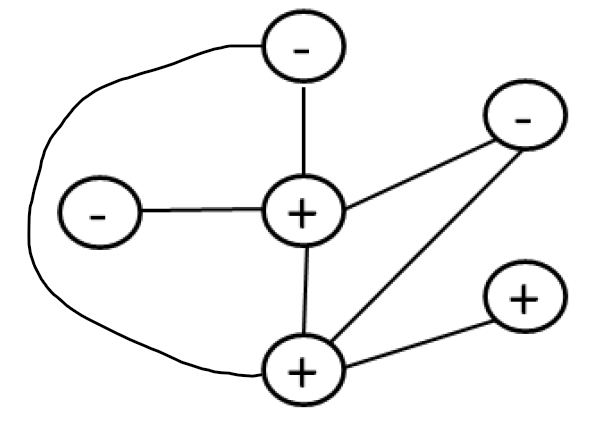
\includegraphics[width=0.5\textwidth]{img/q6.png}
	\end{figure}
	
	
\end{itemize}





\end{document}